\chapter{Is Infrastructure Regional Cement?}

It is widely thought that a modern infrastructure must be a prerequisite for economic development. This belief can be turned into an argument for state control of infrastructure development so as to avoid the occurrence of any regional disparities. Many large plans, both by the British government and the European Development Fund have been formulated based on such a supposition: An example of this is the \textit{Barnes Plan} launched just after the Second World War. Its purpose was to introduce improvements to assist Development Areas in particular and industrial development generally \citep{Rodgers:1959}.

However the nature of the relationship between infrastructure and regional development is not at all clearly understood and consequently the impacts of improvement to an existing stock are not easily assessed. This is especially so when trying to look at the impact of infrastructure developments when regions' infrastructure stocks are not vastly disparate.

This chapter finds that there are two main reasons put forward for boosted spending on infrastructure leading to better regional development. Firstly in areas of very poor infrastructure provision, an increase in spending can result in urbanisation and agglomeration which in themselves provide economics of scale and scope. A second reason is that by reducing transport costs, an economy will restructure itself geographically in order to take advantage of comparative advantages leading to a better allocation efficiency.

However, it goes on to note that current allocational inefficiencies are, however, not usually only caused by lacking infrastructure. Other factors are also in need of improvement. This has been shown empirically by the lack of movement by firms following infrastructure development. Firms claim that the labour force and incentives by regional agencies are more potent lures. The economies of urbanisation are limited. Congestion and other bottlenecks, it seems are more of a worry to firms than basic infrastructure provision. Furthermore infrastructure developments intended to link regions can in reality have perverse affects.
 
A sufficiently established infrastructure can provide any particular location with a productivity bonus. This can be caused by external economies of agglomeration and urbanisation which a good infrastructure facilitates. The high population density makes the supply of public goods services viable: These range from the provision of cheap utilities through to waste removal facilities. Also, allowing easy access between places of work and rest allows people to live further away from industrial areas increasing quality of life \citep{Henderson:1988}.

\begin{figure}
\tikzstyle{arrow} = [thick,->,>=stealth]
\tikzstyle{arrowd} = [thick,dashed,->,>=stealth]
\centering
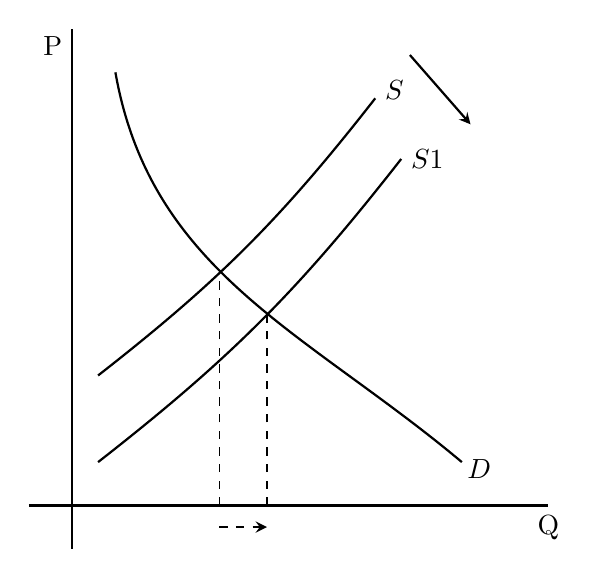
\begin{tikzpicture}[scale=1.1]

% Axis
\draw [thick] (-0.5,-0.0) --(5.5,0);
\draw [thick] (0,-0.5) -- (0,5.5);
\node [left] at (0,5.3) {P};
\node [below] at (5.5,0) {Q};

%Downward slopping line
\draw [thick] (0.5,5) to [out=280,in=140] (4.5,0.5);
\node [above] at (4.7,0.2) {$D$};

% Upward Slopping S1
\draw [thick] (0.3,0.5) to [out=38,in=232] (3.8,4);
\node [right] at (3.8,4) {$S1$};

% Upward Slopping S
\draw [thick] (0.3,1.5) to [out=38,in=232] (3.5,4.7);
\node [right] at (3.5,4.8) {$S$};

% dashed lines
\draw [dashed](1.7,0)--(1.7,2.7);
\draw [dashed](2.25,0)--(2.25,2.3);

\draw [arrow] (3.9,5.2) -- (4.6,4.4);
\draw [arrowd] (1.7,-0.25) -- (2.25,-0.25);

\end{tikzpicture}
  \caption{Benefits of Cheaper Transport}
  \label{fig:cheaper_transport}
\end{figure}


A second reason for increasing prosperity following infrastructure development would be from increased allocational efficiency as production is freed to relocate to areas of increased productivity, from which it had previously been barred by poor connections. This would show itself in cheaper transport facilities lowering the overall cost of production. This will lead to increased profitability which can be represented by the shift in the supply curve from S to Sl in Figure \ref{fig:cheaper_transport}. The figure shows that output will thus increase. There are three conditions that are required for this to be significant:

Firstly there have to be otherwise unemployed resources of the right kind to produce the extra output Secondly transport costs have to be a significant element of total production costs. Finally, the change in transport costs has to be significantly large. Empirical studies do not support these three assumptions. Areas with low levels of development are seldom in the situation of lacking good accessibility only; they have other disadvantages, \textit{exempli gratia:} lack of suitable sites and skilled labour. Transport costs are only between five and ten percent of total production costs. The decrease in transport costs is only a small fraction of existing transport costs: loading times are equally significant \citep{Parkinson:1981}. Not only this, but the local growth has to be sufficiently strong to counter the fact that it is now also cheaper to transport good produced elsewhere to the markets around the infrastructure improvements \citep{Chisholm:1973}.

Further empirical evidence suggests that attempts to encourage regional developments to obtain an equality of opportunity for all its citizens by encouraging growth in relatively backward areas arc flawed: business relocation's following infrastructure reconfigurations tend to be intra-regional rather than inter-regional \citep{Parkinson:1981}. A study of the effects of the building of the M62 by Leeds University showed that the vast majority of the traffic (about 90\%) was simply reassigned from existing roads. The reduction in total production costs of those reassigned to this new motorway, was estimated to be about a third of a percent. This was deemed insignificant \citep{Gwilliam:1978}. A study by Geary and Thomas is more significant for those looking at infrastructures effects on adjoining regions of previously different properties. This looked at the development effect in Wales for the first three years after the opening of the Severn Bridge. It found little evidence of business location decisions being affected by the new infrastructure \citep{Geary:1973}.

Botham carried nut an analysis of the 1957-1972 trunk road programme. The results showed a relatively small (in the order of one hundred thousand jobs) redistribution. Also, other determinants of travel costs such as changes in fuel taxation and legislation on drivers' hours can be as significant as road improvements \citep{Botham:1980}. This is confirmed by a survey of firms (results shown in Table \ref{tab:factors_relocation}) carried out by the Department of Industry which finds firms more concerned with labour availability and regional incentives \citep{Maarquand:1980}.

\begin{longtable}{cccc}
\hline
\textbf{Factor} & \textbf{Major} & \textbf{Minor} & \textbf{No Part}\\ 
\hline
Labour Availability & 69 & 25 & 7 \\
Regional Incentives & 64 & 25 & 12\\
Local Authority Aids & 42 & 36 & 22 \\
Transport Facilities & 42 & 31 & 28 \\
Access to Markets & 32 & 25 & 43 \\
Scarce Skills & 18 & 33 & 49 \\
Environment & 17 & 33 & 50 \\
\hline \\

\caption{Factors affecting firms relocating in Assisted Areas 1972-1976.}  \label{tab:factors_relocation}\\
\end{longtable}




There is some evidence that sites in the vicinity of motorway interchanges are in demand by developers, although it is contended that such developments can be at the expense of nearby inner city areas e.g. M4 and M25 interchanges with respect to Cardiff and London. This is shown in an increase in the level of rents demanded for the first few years after a new road is built. After this rents tend to revert to the regional average \citep{Hillier:1979}. The increases in rents are however small compared to geographic distance from London:

\begin{displayquote}
Of the factors considered, it seems that motorways, new towns, good accessibility and ports do not, by themselves, cause high rents. None of these factors compare with the dominating effect of London. Distance from London seems clearly to be the most important locational factor affecting industrial rents \citep{Hillier:1980}.
\end{displayquote}

Given the lack of interest in basic infrastructure shown by commerce and the limited nature of resources available to a government there is a question of where to provide new infrastructure: provision in advance of demand for its use in certain lagging regions has to be weighed against the lack of provision in areas of real demand and immediate utilisation.

In a 1989 survey of the views of businesses by the Department of Transport, road transport and communications were put forward as being of paramount importance to the overwhelming majority of establishments surveyed. However the complaints were not from the NorthEast which has a sparse infrastructure base, but from the South-East. The main cause of this is the increasing number of bottlenecks blocking goods movements and causing problems for the labour forces attempts to travel to and from work in the morning \citep{DTI:1989}.

Vickerman confirms this analysis, referring to the the results of Biehl's analysis of the limiting effect on output played by poor infrastructure in the European Community \citep{Biehl:1991}. He found both over and under-utilisation. The two regions that showed the most obvious over utilisation of infrastructure are the south-east of England and the Nord-Pas de Calais region of France. This reinforces the view that regions with large amounts of infrastructure are as likely to suffer from infrastructure problems. The lesser developed regions often show under utilisation of infrastructure. This is likely to be the result of the heavy investment of the European Regional Development Fund in infrastructure in an attempt to bring behind regions in line with the rest of Europe \citep{Vickerman:1994}.

Increased spending on infrastructure it seems can have a perverse effect on regional growth. An example of this is the High Speed Train Network being build across Europe. Recent, major strides in the development of high-speed rail services in Europe have caught the attention of bureaucrats who saw one pan-European railway network as having huge integrative potentiaL Far-reaching plans have been made for a Europe-wide High Speed Train Network extending some 35.000 km including some 20,000 km of new dedicated track, and reaching all the current EU member states and eventually eastern Europe as well \citep{Ross:1994}.

Expectations of High Speed Train Technology are high: One assumption is that rapid rail technologies will have a regenerative effect for the European rail industry, and more widely for overall transport networks via inter-modal linkages \citep{EC:1990}. A second reason for high expectations is the belief that the network will lead to an injection of capital and employment opportunities through regional development. A third belief is that the network will lead to harmonisation of goods and people carriers across the EU, following the underlying principle of the single market \citep{Ross:1994}.

There is however a problem. Firstly, the experience of HST lines that are already operational is mixed. Although the French TGV operates at a fifteen percent profit and British Rail's Intercity network has been successfully privatised, Spain's Madrid-Seville AVE line has had far more mixed results. To be financial viable, HST lines need to cover medium distance travel (200-500 km) and serve large populations at each end, with high market demand and journey times under fours hours in order to keep competitive with airlines \citep{Blum:1992}. Such conditions exist in the Low Countries, France and Germany, but rapidly deteriorate in the peripheral regions. This is likely to lead to a two tier system of transport infrastructure. Worse, HSTs draw in valuable funds: Even in a rich country like France, the heavy costs of the TGV development have been widely blamed for the relative backwardness of its regional rail systems, particularly in the South \citep{Vickerman:1990}.

In this chapter we have looked at the argument that infrastructure development can lead to large changes in regional growth, and that therefore infrastructure development should be controlled by the state. The two reasons for the association of regional growth and infrastructure, urbanisation and increased allocational efficiency, have been presented and shown to be of little empirical value. Firms have not moved and rents have changed little (after short term shifts) according to changes in infrastructure in remote regions.

In fact most complaints about infrastructure come from well developed areas which have grown so excessively densely populated that congestion and other bottlenecks have formed. Government intervention to improve backward regions prosperity can thus not be justified, indeed intervention in the form of the European High Speed Train Network has been shown to damage backward regions. Again the market should be left alone.